\subsection{Summierte Quadratur}

\begin{Definition}{quadratur}
  Eine \define{Quadraturformel} $Q_{[a,b]}(f)$ ist eine Approximation
  des Integrals
  \begin{gather}
    Q_{[a,b]}(f) \approx \int_a^b f(x)\dx
  \end{gather}
  in der Form
  \begin{gather}
    Q_{[a,b]}(f) = \sum_{i=0}^n \omega_i f(x_i).
  \end{gather}
  Die Stützstellen $x_i$ bezeichnen wir auch als
  \define{Quadraturpunkte}, die Zahlen $\omega_i$ als
  \define{Quadraturgewichte}.
\end{Definition}

\begin{Definition}{quadratur-summiert}
  Ist eine Quadraturormel bezüglich einer Zerlegung
  $\mathcal I_h$ des Intervalls $[a,b]$ in der Form
  \begin{gather}
    Q_{[a,b]}(f) = \sum_{i=1}^n Q_{I_i} (f)
  \end{gather}
  definiert, so sprechen wir von \textbf{summierter},
  \textbf{iterierter} oder \textbf{stückweiser Quadratur}.
\end{Definition}

\begin{Satz}{quadratur-kondition}
  Die Integration einer Funktion $f\in C[a,b]$ über das Intervall $[a,b]$ genügt der Konditionsabschätzung
  \begin{gather}
    \left|\int_a^b f(x)\dx \right| \le \kappa_{\text{abs}} \max_{x\in[a,b]}\abs{f(x)},
    \qquad \kappa_{\text{abs}} = b-a.
  \end{gather}
  Für die Quadraturaufgabe gilt
  \begin{gather}
    \left| Q_{[a,b]}(f)\right| \le \kappa_{\text{abs}} \max_{x\in[a,b]}\abs{f(x)},
    \qquad \kappa_{\text{abs}} = \sum_i \abs{\omega_i}.
  \end{gather}
\end{Satz}

\begin{Definition}{quadratur-lokale-fehlerordnung}
  Gilt bei einer summierten Quadraturformel die Abschätzung
  \begin{gather}
    \left|\int_{I_i} f(x)\dx - Q_{I_i}(f)\right|
    =\bigo\left(h_i^{k+1}\right)
  \end{gather}
  für jedes Teilintervall $I_i$ und Funktionen $f\in C^{k+1}[a,b]$, so
  sprechen wir von der \textbf{lokalen
    Fehlerordnung}\defindex{Fehlerordnung}\defindex{lokale Fehlerordnung} $k+1$.
\end{Definition}

\begin{Satz}{summierte-quadratur}
  Sei $\mathcal I_h$ eine Zerlegung von $[a,b]$ der Feinheit $h$ und
  $c_q$ sei so gewählt, dass
  \begin{gather}
    c_q \min_{I_i\in \mathcal I_h} h_i \ge h.
  \end{gather}
  Sind dann die Formeln $Q_{I_i}$ von lokaler Fehlerordnung $k+1$ für
  $f\in C^{k+1}[a,b]$, so gilt für die summierte Quadratur $Q_{[a,b]}$
  die Abschätzung
  \begin{gather}
    \left|\int_a^b f(x)\dx - Q_{[a,b]}(f)\right|
    = \mathcal O\left(h^{k}\right).
  \end{gather}
\end{Satz}

\begin{proof}
  Das kleinste Intervall hat die Länge $h/c_q$. Damit ist die Anzahl
  der Intervalle beschränkt durch $n_{\max}=c_q (b-a)/h$. Aus der
  lokalen Fehlerordnung ergibt sich die Existenz einer Konstanten $c$,
  so dass
  \begin{gather}
    \left|\int_{I_i} f(x)\dx - Q_{I_i}(f)\right| \le c h_i^{k+1}.
  \end{gather}
  Damit schätzen wir ab
  \begin{align}
    \left|\int_a^b f(x)\dx - Q_{[a,b]}(f)\right|
    &= \sum_{I_i\in\mathcal I_h}  \left|\int_{I_i} f(x)\dx - Q_{I_i}(f)\right|\\
    &\le \sum_{I_i\in\mathcal I_h} c h^{k+1}\\
    & \le n_{\max} c h^{k+1} = \bigo\left(h^{k}\right).
  \end{align}
\end{proof}

\subsection{Quadratur auf Einzelintervallen}

\begin{Notation}{quadrature}
  In diesem Abschnitt integrieren wir wieder über das Intervall
  $I=[a,b]$, aber mit dem Gedanken, dass es sich eigentlich um die
  Teilintervalle $I_i$ einer summierten Quadratur handelt.

  Wir betrachten in der Regel Quadraturformeln mit $n$ Punkten
  $x_1,\dots,x_n$. Oft benutzen wir Ergebnisse aus den Abschnitten
  über Interpolation. Dabei ist jeweis darauf zu achten, dass die
  Indizes dort bei null loslaufen. Der Grund für diesen wechsel ist,
  dass wir bei der Interpolation den Grad der Polynome als führende
  Größe angesehen haben, während hier die Anzahl der Quadraturpunkte
  im Vordergrund steht.
\end{Notation}

\begin{Definition}{grad-exaktheit}
  Eine Quadraturformel $Q_I$ heißt \define{exakt vom Grad $k$} und $k$
  heißt der \define{Grad der Exaktheit} von $Q_I$, wenn sie exakt für
  alle Polynome vom Grad bis zu $k$ ist, also
  \begin{gather}
    \int_I p(x)\dx - Q_{I}(p) = 0 \qquad \forall p\in \P_k.
  \end{gather}
\end{Definition}

\begin{remark}
  Als unmittelbare Folgerung erhalten wir für jede Quadraturformel,
  die mindestens exakt fom Grad null ist, dass
  \begin{gather}
    \sum \omega_i = b-a.
  \end{gather}
\end{remark}

\begin{Lemma}{exakt-ordnung}
  Sei die Quadraturformel $Q_I$ exakt vom Grad $k$ und
  $\abs{I} \le h$. Dann gilt für $f\in C^{k+1}(I)$
  \begin{gather}
    \left|\int_{I} f(x)\dx - Q_{I}(f)\right| = \bigo\bigl(h^{k+2}\bigr)
  \end{gather}
\end{Lemma}

\begin{remark}
  Die Überlegungen des vorhergehenden Lemmas sind insbesondere dann
  nützlich, wenn man die Konvergenzordnung einer Methode schnell
  überschlagen möchte. Man spart sich auf diese Art genauere
  Untersuchungen der Fehlerdarstellung. Umgekehrt sind die Konstanten
  in den Abschätzungen auch scharf und die Analysis erhebt auch nicht
  den Anspruch. Im Detail werden wir daher auch noch schärfere
  Abschätzungen machen.
\end{remark}

\begin{Definition}{interpolatorische-quadratur}
  Eine \define{interpolatorische Quadraturformel} mit $n$
  Quadraturpunkten $x_1,\dots,x_n$ approximiert das Integral einer
  Funktion $f$ durch das exakte Integral ihres Interpolationspolynoms
  $p\in \P_{n-1}$
\end{Definition}

\begin{Lemma}{interpolatorisch-omega}
  Seien $x_1,\dots,x_n$ die Quadraturpunkte einer interpolatorischen
  Quadraturformel $Q_I$, die exakt für Polynome vom Grad $n-1$
  ist. Dann sind die Gewichte gegeben durch
  \begin{gather}
    \omega_i = \int_I \plagrange_{i;x_1,\dots,x_n}(x)\dx,
  \end{gather}
  wobei $\plagrange_{i;x_1,\dots,x_n}$ das
  Lagrange-Interpolationspolynom zum Punkt $x_i$ ist.
\end{Lemma}

\begin{proof}
  Die Lagrange-Polynome $\plagrange_i$ sind Polynome vom Grad
  $n-1$. Es gilt daher
  \begin{gather}
    \int_I \plagrange_i = \sum_{k=1}^n \omega_k \plagrange_i(x_k) = \omega_i.
  \end{gather}
\end{proof}

\begin{Definition}{newton-cotes}
  Werden die Quadraturpunkte $a=x_1,\dots,x_n=b$ gleichmäßig im
  Intervall $[a,b]$ verteit, so spricht man von einer
  \define{Newton-Cotes-Formel}. Die
  ersten drei klassischen Formeln sind auf dem Einheitsintervall
  $[0,1]$ gegeben durch
  \begin{center}
    \begin{tabular}{l|c|cccc|cccc}
      & $n$ & \multicolumn{4}{|c}{$x_i$} & \multicolumn{4}{|c}{$\omega_i$}
      \\\hline
      Trapezregel & 2 & 0 & 1 &&& \nicefrac12 & \nicefrac12\\
      Simpson-Regel\footnote{Auch Keplersche Fassregel} & 3 & 0 & \nicefrac12 & 1 &
                          & \nicefrac16& \nicefrac46& \nicefrac16\\
      \nicefrac38-Regel\footnote{Von Newton auch mit dem Adjektiv \glqq pulcherrima\grqq{} belegt.}
      & 4 & 0 & \nicefrac13 & \nicefrac23 & 1
                          & \nicefrac18& \nicefrac38& \nicefrac38& \nicefrac18
    \end{tabular}
  \end{center}
\end{Definition}

\begin{remark}
  Genauer gesagt handelt es sich bei den Formeln in
  \slideref{Definition}{newton-cotes} um \textbf{geschlossene}
  Newton-Cotes-Formeln, die die Intervallenden als Quadraturpunkte
  enthalten.  Bei offenen Formeln sind die Intervallenden keine
  Quadraturpunkte. Während offene Newton-Cotes-Formeln von geringem
  Interesse sind, werden wir später bei der Gauß-Quadratur offene
  Formeln kennenlernen.

  Summierte geschlossene Formeln werden of direkt als Summe über die
  Zerlegung geschrieben. Dazu numerieren wir nun alle Stützpunkte der
  Reihe nach, egal ob es sich um Intervallenden oder innere
  Stützpunkte handelt von 1 bis $n$. Sei $h$ nun der Abstand zweier Quadraturpunkte
  der summierten Formel. dann gilt für die summierte Trapezregel
  \begin{gather}
    Q(f) = h\left(\tfrac12 f_1 + f_2 +\dots+f_{n-1}+\tfrac12 f_n\right).
  \end{gather}
  Bei der summierten Simpson-Regel (man beachte die Umskalierung der Intervall-Länge) ergibt sich
  \begin{gather}
    Q(f) = \tfrac h3\left(f_1 + 4 f_2 + 2 f_3 + 4 f_4 + 2 f_5
      + \dots + 2 f_{n-2} + 4 f_{n-1} + f_{n}\right).
  \end{gather}
  Der Aufwand für Funktionsauswertungen in den Intervallenden halbiert
  sich bei dieser Darstellung der summierten Regeln. Natürlich lassen
  sich die summierten Formeln für Intervalle wechselnder Länge
  umschreiben. Bei der Simpson-Regel muss man aber dabei Bedenken,
  dass immer 2 Subintervalle ein Intervall der Zerlegung ergeben.
\end{remark}


\begin{Satz}{newton-cotes-error}
  Die Fehler der Newton-Cotes-Formeln auf dem Intervall $I$ der Länge
  $h$ lassen sich wie folgt abschätzen
  \begin{gather}
    \left|\int_I f\dx - Q_I(f)\right| \le
    \begin{cases}
      \dfrac{h^3}{12}\max\limits_{\xi\in I}\abs{f''(\xi)}
      &\text{Trapezregel}\\
      \dfrac{h^5}{2880}\max\limits_{\xi\in I}\abs{f^{(4)}(\xi)}
      &\text{Simpson-Regel}\\
      \dfrac{h^5}{6480}\max\limits_{\xi\in I}\abs{f^{(4)}(\xi)}
      &\text{\nicefrac38-Regel}
    \end{cases}
  \end{gather}
\end{Satz}

\begin{proof}
  Der Beweis für die Trapezregel und die \nicefrac38-Regel benutzt
  Interpolation in den Quadraturpunkten und die Fehlerdarstellung des
  Interpolationsfehlers. Für die Trapezregel ist er als Hausaufgabe
  gestellt.

  Hier führen wir nur den Beweis für die Simpson-Regel. Nachdem man
  experimentell beobachtet, dass die Formel exakt vom Grad 3 ist,
  nicht vom erwarteten Grad 2, konstruieren wir eine Interpolation auf
  $I=[x_1,x_3]$ mit Mittelpunkt $x_2$ wie folgt:
  \begin{xalignat}2
    p(x_1) &= f(x_1) & p(x_2) &= f(x_2) \\
    p(x_3) &= f(x_3) & p'(x_2) &= f'(x_2).
  \end{xalignat}
  Die letzte Bedingung ist aus der Quadraturformel nicht
  ersichtlich. Folgen wir jedoch der Basiskonstruktion im
  \slideref{Satz}{hermite-interpolation} über die Wohlgestelltheit der
  Hermite-Interpolationsaufgabe, so erhalten wir
  \begin{xalignat}2
    H_{10}(x) &= \tfrac{4(x-x_2)^2(x_3-x)}{h^3}&
    H_{20}(x) &= \tfrac{4(x-x_1)(x-x_3)}{h^2}\\
    H_{30}(x) &= \tfrac{4(x-x_2)^2(x-x_1)}{h^3}&
    H_{21}(x) &= \tfrac{4(x-x_2)(x-x_1)(x-x_3)}{h^2}
  \end{xalignat}

  \begin{figure}[tp]
    \centering
    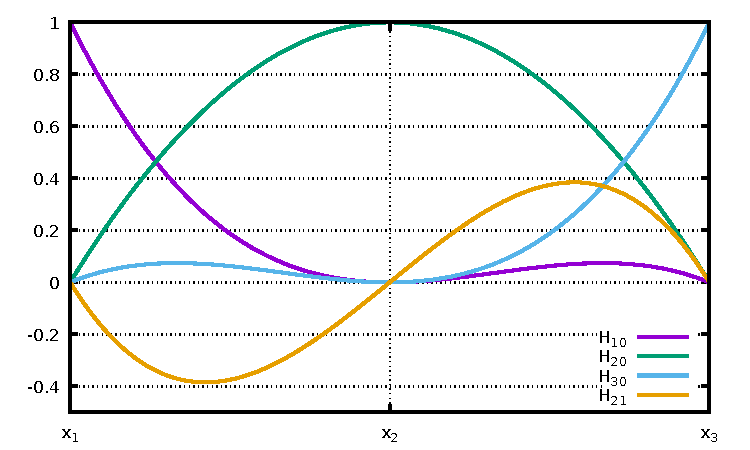
\includegraphics[width=.8\textwidth]{graph/interpolation/simpson}
    \caption{Basisfunktionen für die Simpsonregel. Beachte, dass $H_21$ in allen Quadraturpunkten verschwindet und auch das Integral null ist.}
    \label{fig:simpson}
  \end{figure}
  Die Funktion $H_{21}(x)$ ist das Produkt der Parabel
  $(x-x_1)(x-x_3)$, die symmetrisch zur Intervallmitte ist mit einer
  linearen Funktion mit Nullstelle in der Intervallmitte. Daher
  verschwindet ihr Integral und das zugehörige Integrationsgewicht ist
  null. Die Simpson-Regel lässt sich also schreiben als
  \begin{gather}
    Q_I = \frac h6f(x_1)+\frac{4h}6f(x_2) + \frac h6f(x_3) + 0 f'(x_2).
  \end{gather}
  Für die obige Interpolation gilt nach
  \slideref{Satz}{Hermite-restglied} die Fehlerdarstellung
  \begin{gather}
    f(x) - p(x) = \frac{f^{4}(\xi(x)}{4!} \pnewton_{x_1,x_2,x_2,x_3}(x).
  \end{gather}
  Integration ergibt
  \begin{align}
    \left|\int_I f\dx - Q_I(f)\right|
    &= \left|\int_I \bigl(f(x) - p(x)\bigr)\dx\right|\\
    &\le \max_{\xi\in I} \frac{f^{4}(\xi}{4!}
      \int_I \pnewton_{x_1,x_2,x_2,x_3}(x) \dx.
  \end{align}
  Schließlich berechnen wir
  \begin{gather}
    \int_I \pnewton_{x_1,x_2,x_2,x_3}(x) \dx
    = \int_I (x-x_1)(x-x_2)^2(x-x_3)
    = \frac1{120}
  \end{gather}
\end{proof}

\begin{remark}
  Die Newton-Cotes-Formel mit 9 Punkten hat negative Gewichte, was
  auch bei höheren Formeln wieder auftritt. Bei solchen Formeln wird
  die Konditionierung der Quadraturaufgabe schlechter als die der
  Integration. Auch kann es sein, dass eine nirgendwo negative
  Funktion durch eine solche Quadratur ein negatives Integral erhält.
  Deswegen werden solche Formeln nicht verwendet.
\end{remark}

\subsection{Gauß-Quadratur}

\begin{Lemma}{quadratur-exakt-max}
  Sei $Q_n$ eine Quadraturformel auf einem Intervall $I$ mit $n$
  Quadraturpunkten. Dann ist $Q_n$ maximal exakt vom Grad $2n-1$.
\end{Lemma}

\begin{proof}
  Siehe \cite[Satz 3.1]{Rannacher17}
\end{proof}

\begin{Definition}{Gauss-Legendre}
  Die $n$-Punkt-\define{Gauß-Legendre-Formel} auf dem Intervall
  $I=[-1,1]$ benutzt als Stützstellen $x_1,\dots,x_n$ die Nullstellen
  des Legendre-Polynoms $\plegendre(x)$ vom Grad $n$. Ihre
  Quadraturgewichte sind die Integrale der Lagrange-Polynome
  \begin{gather}
    \omega_i = \int_I \plagrange_{i;x_1,\dots,x_n}(x)\dx.
  \end{gather}
\end{Definition}

\begin{Satz}{gauss-legendre}
  Die $n$-Punkt-Gauß-Legendre-Formel ist wohldefiniert und exakt für
  beliebige Polynome vom Grad $2n-1$.
\end{Satz}

\begin{Satz}{gauss-legendre-eindeutig}
  Seien die Quadraturformeln $Q_k$ mit Quadraturpunkten
  $x_1^{(k)},\dots,x_k^{(k)}$ für $k=1,\dots,n$ auf dem Intervall
  $I=[-1,1]$ exakt für beliebige $p\in \P_{2k-1}$. Dann sind die
  Polynome
  \begin{gather}
    p_k(x) = \prod_{i=1}^k (x-x_i^{(k)}) \in \P_k
  \end{gather}
  und $p_0(x) = 1 \in \P_0$ paarweise orthogonal bezüglich des
  $L^2$-Skalarprodukts. Insbesondere sind sie damit Vielfache der
  Legendre-Polynome $\plegendre_k$ und die
  $n$-Punkt-Gauss-Legendre-Formel ist die einzige Formel mit $n$
  Punkten, deren Grad der Exaktheit $2n-1$ ist.
\end{Satz}

\begin{Lemma}{gauss-legendre-gewichte}
  Die Gewichte der Gauss-Legendre-Formeln sind positiv und genügen der
  Darstellung
  \begin{gather}
    \omega_i = \int_{-1}^1 \prod_{j\neq i}
    \left(\frac{x-x_j}{x_i-x_j}\right)^2\dx.
  \end{gather}
\end{Lemma}

\begin{Lemma}{gauss-legendre-fehler}
  Für die Gauss-Legendre-Formel mit $n$ Quadraturpunkten auf
  $I=[-1,1]$ gilt die Fehlerabschätzung
  \begin{gather}
    \left|\int_I f\dx - Q_n(f)\right|
    \le \max_{\xi\in I}\frac{f^{(2n)}(\xi)}{(2n)!}
    \int_{-1}^1 \prod_{i=1}^n(x-x_i)^2.
  \end{gather}
\end{Lemma}

\begin{remark}
  Alle Resultate dieses Abschnitts gelten für Skalarprodukte der Form
  \begin{gather}
    \scal(p,q) = \int_I \omega(x)p(x)q(x)\dx
  \end{gather}
  mit einer positiven Gewichtsfunktion $\omega(x)$, wenn man die
  Legendre-Polynome durch die entsprechenden orthogonalen Polynome
  ersetzt.
\end{remark}

\subsection{Richardson-Extrapolation und Romberg-Quadratur}

\begin{Definition}{richardson-extrapolation}
  Sei $T(h)$ eine numerische Methode zur Approximation des
  tatsächlichen Wertes $T(0)$ mit Diskretisierungsparameter $h$ und
  Fehlerabschätzung $\abs{T(h)-T(0)} = \bigo(h^p)$. Zur
  \define{Richardson-Extrapolation} wertet man diese Methode mit einer
  Schrittfolge $h_1, h_2,\ldots,h_n$ aus, so dass die Schrittweite
  (theoretisch) gegen null geht. Wertet man dann das
  Interpolationspolynom $p(h^p)$ an der Stelle $h=0$ aus, so bekommt
  man unter stärkeren Voraussetzungen die verbesserte Approximation
  \begin{gather}
    \abs{T(0)-p(0)} = \bigo(h^{np}).
  \end{gather}
\end{Definition}

\begin{remark}
  Tatsächlich genügt die einfache Fehlerabschätzung
  $\abs{T(h)-T(0)} = \bigo(h^p)$ nicht, um die behauptete
  Konvergenzordnung zu beweisen. Man benötigt eine asymptotische
  Fehlerentwicklung der Form
  \begin{gather}
    T(h)-T(0) = \tau_1 h^p + \tau_2 h^{2p} + \dots \tau_n h^{np}
    + \bigo(h^{(n+1)p}).
  \end{gather}
\end{remark}

\begin{Definition}{Romberg-quadratur}
  Die \define{Romberg-Quadratur} beruht auf einer summierten
  Quadraturformel $Q_h$ der Ordnung $h^p$, die für eine Folge von
  Schrittweiten $h_1,\dots, h_n$ angewandt wird. Aus diesen berechnet
  man mit dem \putindex{Neville}-Algorithmus Approximationen für
  $Q_0$.
\end{Definition}

\begin{Algorithmus*}{romberg}{Romberg-Quadratur}
  \lstinputlisting{code/romberg.py}
\end{Algorithmus*}

\subsection{Praktische Aspekte}

\begin{remark}
  Die Konvergenzabschätzungen der Form
  \begin{gather}
    \left|\int_I f\dx - Q_h(f)\right| \le c h^p \norm{f^{p+1}}_{\infty;I}
  \end{gather}
  verlieren ihren Nutzen für große $h$, wenn die Ableitungen von $f$
  wachsen. Schlimmstenfalls bekommt man dann aus der
  Interpolationseigenschaft noch immer
  \begin{gather}
    \left|\int_I f\dx - Q_h(f)\right| \le c \norm{f}_{\infty;I}.
  \end{gather}
  Es gibt aber keine Garantie, dass der Fehler bei feinerer
  Unterteilung schrumpft.
  
  Ist aber $f\in C^{p+1}(I)$, so gilt die obige Abschätzung für
  hinreichend kleine $h_1>h_2$ in der stärkeren Form
  \begin{gather}
    \left|\int_I f\dx - Q_{h_2}(f)\right|
    \approx \left(\frac{h_2}{h_1}\right)^p
    \left|\int_I f\dx - Q_{h_1}(f)\right|.
  \end{gather}
  Man spricht hier vom asymptotischen Bereich, für größere $h$ vom
  präasymptotischen Bereich.
\end{remark}

%%% Local Variables:
%%% mode: latex
%%% TeX-master: "main"
%%% End:
